\documentclass[a4paper]{article}

\usepackage[UKenglish]{babel}
\usepackage[T1]{fontenc}
\usepackage{microtype}

\usepackage{graphicx}
\usepackage{geometry}

\usepackage{csquotes}

\ExplSyntaxOn
\NewDocumentCommand\acro{m}{\textsc{\tl_lower_case:n{#1}}}
\ExplSyntaxOff
\NewDocumentCommand\email{m}{\href{mailto:#1}{#1}}
\NewDocumentCommand\foreign{m}{\textit{#1}}
\NewDocumentCommand\pkg{m}{\textsf{#1}}

\usepackage{hyperref}
\hypersetup{hidelinks}

\author{Joseph Wright\thanks{\email{joseph.wright@morningstar2.co.uk}}}
\date{March 2021}
\title{The \url{learnlatex.org} project\\Grant report to UK-TUG}

\begin{document}

\maketitle

\section{Introduction}

As described in the proposal for the \url{learnlatex.org} site, the project is
focussed on creating an interactive website to allow new users to learn to use
\LaTeX{} as a document preparation tool. The aims were
\begin{enumerate}
  \item To focus on key topics for most new users
  \item To allow users to try code examples directly in the website
  \item To ensure that the material was up-to-date and promoted
    best practice
  \item To ensure that the wider community can update the content
  \item To present the material in site following current web design
    best practice
\end{enumerate}

Funding was agreed with UK-TUG to support the last point. In contrast to the
other aspects of the project, this area is outside the expertise of the team
behind the site. Moreover, there are a large number of consultants who
specialise in web development, and it was felt that therefore, this aspect of
the work would be best handled using an external paid expert.

Here, we will summarise the work which has occured on the site whether funded
by UK-TUG or otherwise.

\section{Content development}

A GitHub organisation was established to build the content and ultimately to
use GitHub Pages to host the site. Around a dozen contributors were then
approached to seek input into the material. Promotion \foreign{via} Twitter and
on TeX StackExchange led to additional contributors either joining the core
team or making focussed contributions.

The starting point for content creation was the existing UK-TUG training
materials, originally developed by Nicola Talbot. Discussion within the writing
team led to some reordering of topics. The original vision was to have around a
dozen topics. This has expanded to $16$ main lessons in the live site.

In working on the content, it became apparent that there was a need to have
both a core set of lessons and a parallel set of additional pages. The latter
take the same idea as their \enquote{parent} page and introduce additional
detail. This has allowed us to cover a large amount of material whilst avoiding
overloading new users. For example, presentations using \pkg{beamer} are not
vital for all users, so are covered in an additional lesson rather than
the main lesson on document classes.

The second aspect which became apparent during content development was that
focussing purely on English would be limiting. We therefore adjusted the site
structure, such that it now allows multiple languages to be featured. This work
overlapped with input from the web developer (see below). This work has
resulted in
\begin{itemize}
  \item English
  \item Spanish
  \item French
  \item Portuguese
  \item Vietnamese
  \item Trukish
  \item Marathi
\end{itemize}
translations being available in full. Other translations are in progress but
are not currently live.

Translations also raised the question of language-specific guidance, for
example to cover \pkg{babel} features, use of specialist fonts, \foreign{etc.}
Again, this has been integrated into the site structure.

\section{Online compilation}

David Carlisle has led efforts to develop suitable online compilation support
for the site. He initially explored a number of third-party set ups, which were
useful for development but which presented challenges in terms of installation
version, support for \foreign{e.g.}~up-\TeX{} and other tools. He therefore
established a secondary site, \url{latexcgi.xyz}. This provides online
compilation and returns a PDF. The latter is set up to display using
\texttt{PDF.js}, as this is the best approach for inline display in a
cross-platform way. At present, this web service is running on a low-cost
platform. Future funding support may be required as the site becomes more
widely used: this will be handled in separate applications to relevant bodies.

To support compilation, David has also set up in-place editing of the code
examples in the site. This again uses standard web tools and means that a user
can try all of the examples and questions without needing a local installation
or an account with any site.

In parallel to the in-place set up, we have also worked with Overleaf to ensure
that it is possible to use the examples directly on that site. This works using
their public \acro{api} and so requires no support beyond that documented
interface.

\section{Site development}

Web development, including graphical design and more fundamental structural
work, was carried out by Jonas Jared Jacek (\url{https://www.jonas.me/}). The
initial web design was based on a simple GitHub Pages template. Jonas developed
the current appearance (Figure~\ref{fgr:site}), which is designed following
current \enquote{responsive} web standards.
\begin{figure}
  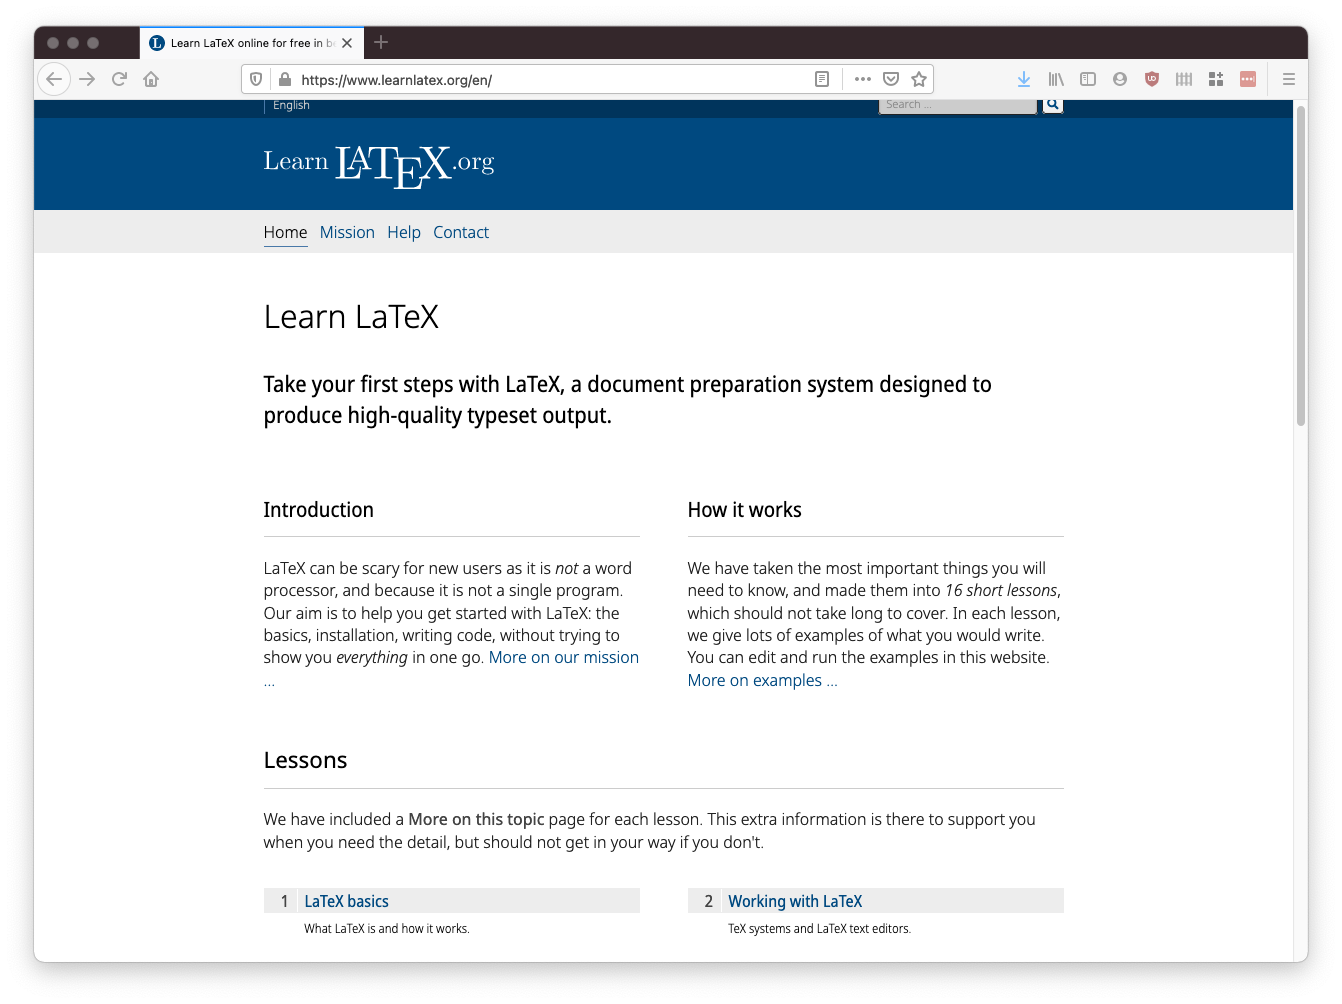
\includegraphics[width = \textwidth]{learnlatex-screenshot}
  \caption{Main page of the \url{learnlatex.org} site in English.\label{fgr:site}}
\end{figure}

The development work ranged over several different areas. Jonas made
suggestions about structure, provided text for some non-technical parts of the
site, handled technical aspects of the underlying structure and carried out
design work. This was an interactive process in consultation with the project
leads. Jonas was particularly keen to work on the multi-lingual aspects of
the site, which arose after he was engaged and a budget was agreed.

\section{Conclusions}

Work on \url{learnlatex.org} has proceeded largely as projected. The site is
now live in seven languages and we are seeing a flow of users. Promotion is
ongoing, including an upcoming guest blog post to Overleaf. The costs of the
site itself are now covered; future funding may be needed to support online
compilation but not for the core content.

\end{document}